\chapter{Performance Analysis}
\label{cha:pa}

In this chapter, we will examine the project's performance. Firstly, we will see
the difference in execution time between a secured binary and a non-secure one.
Secondly, we will see the difference in size between the binaries. Lastly, we will
see an analysis of the obtained results as well as some optimization ideas to further
improve the performance of the project.

To perform a correct analysis of the performances of the project regarding the execution
time we compiled and run $13$ algorithms plus $4$ variations with indirect jumps.
All tests have been conducted on the aforementioned Espressif's board.

\section{Time Performances}
\label{sec:pa_time}

In this section, we will see how the project affects the execution time of the
code (test results can be seen in Figure 5.3). (test result can be seen in
Figures \ref{fig:lowtime} and \ref{fig:hightime}).

As we can see in Table \ref{tab:times}, in most cases the time overhead is not
significant as it affects the fourth or fifth digit.

It is straightforward to understand why this happens for algorithms like \textit{Binary
Search} and \textit{Duff's Device} since we perform few jumps and most of the
computation is performed inside a loop so, the overhead given by the instrumentation
is unnoticeable if compared to the total execution time.

Instead, examples like \textit{Prime} and \textit{Recursive} are a bit trickier.
Since these algorithms work with a recursive approach we expect to perform many jumps
and, as a consequence, we expect the time required for the context switch and the
edge controls to be somewhat impactful. However, results show that even in these
cases the difference is barely noticeable. This could be due to the processor's
frequency which, in the case of Espressif's ESP32-C3, is $160$MHz. This means
that even if we add many instructions the processor is still able to perform
them in a similar time. For example, the \textit{Recursion} algorithm performs around
$4000$ jumps and $4000$ returns which translates to around $8000$ controls and $1
6000$ context switches. However, if we compare those numbers to the $160$ million
operations that the processor can perform in a second we see why the time overhead
is so small.

A peculiar case is the one of the \textit{Fibonacci} algorithm, in this case, we
can see that the overhead is enormous ($1523.24\%$). The possible reason for this
is that this algorithm makes two recursive calls each time so we end up with a staggering
amount of jumps and returns. This leads to many controls and the execution is
strongly affected by this.

These results show that the instrumentation's time overhead is almost
unnoticeable in many cases. However, depending on the algorithm it could affect
the performances heavily.

\begin{figure}[htbp]
  \centering
  \def\stackalignment{r}\stackunder{ 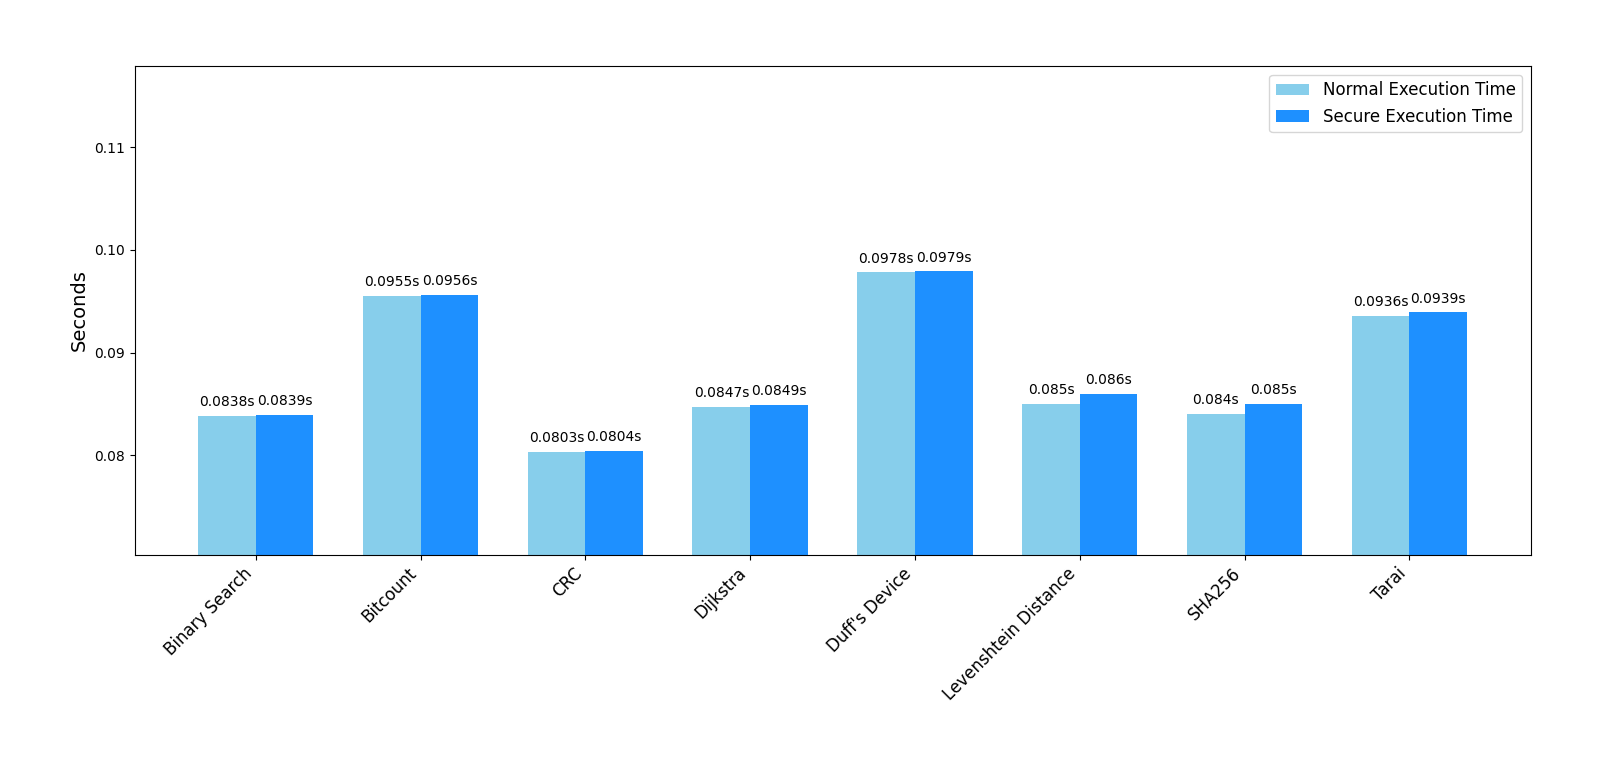
\includegraphics[width=.9\linewidth]{images/low_execution.png} } %
  {\scriptsize }
  \caption{Low execution times}
  \label{fig:lowtime}
\end{figure}

\begin{figure}[htbp]
  \centering
  \def\stackalignment{r}\stackunder{ 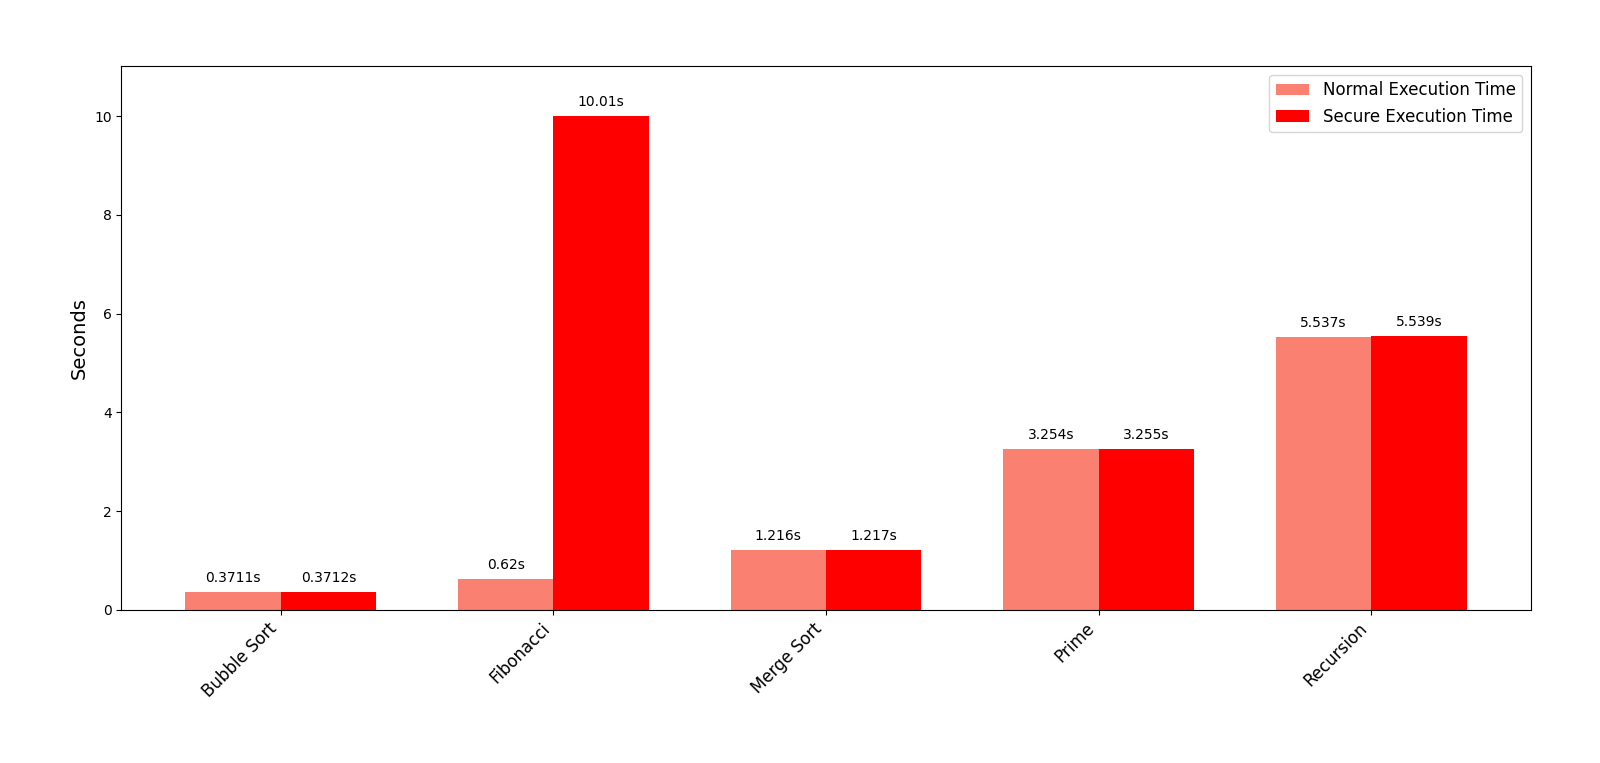
\includegraphics[width=.9\linewidth]{images/high_execution.png} } %
  {\scriptsize }
  \caption{High execution times}
  \label{fig:hightime}
\end{figure}

\begin{table}
  \centering
  \begin{tabular}{|c|c|c|c|}
    \hline
    \textbf{Algorithm}   & \textbf{Normal run time (s)} & \textbf{Secure run time (s)} & \textbf{Time Overhead} \\
    \hline
    Binary Search        & 0.08387                      & 0.08388                      & $0.012\%$              \\
    \hline
    Bitcount             & 0.0955                       & 0.0956                       & $0.11\%$               \\
    \hline
    Bubble Sort          & 0.37113                      & 0.37116                      & $0.008\%$              \\
    \hline
    CRC                  & 0.08025                      & 0.08026                      & $0.012\%$              \\
    \hline
    Dijkstra             & 0.0847                       & 0.0849                       & $0.236\%$              \\
    \hline
    Duff's Device        & 0.097795                     & 0.097799                     & $0.0041\%$             \\
    \hline
    Fibonacci            & 0.6166                       & 10.0089                      & $1523.24\%$            \\
    \hline
    Fibonacci Indirect   & 0.0849                       & 0.1511                       & $77.97\%$              \\
    \hline
    Levenshtein Distance & 0.085                        & 0.086                        & $1.176\%$              \\
    \hline
    Merge Sort           & 1.216                        & 1.217                        & $0.0822\%$             \\
    \hline
    Merge Sort Indirect  & 1.2168                       & 1.2169                       & $0.0082\%$             \\
    \hline
    Prime                & 3.254                        & 3.255                        & $0.03\%$               \\
    \hline
    Prime Indirect       & 3.253                        & 3.254                        & $0.03\%$               \\
    \hline
    Recursion            & 5.537                        & 5.539                        & $0.036\%$              \\
    \hline
    Recursion Indirect   & 5.537                        & 5.539                        & $0.036\%$              \\
    \hline
    SHA256               & 0.084                        & 0.085                        & $1.19\%$               \\
    \hline
    Tarai                & 0.0936                       & 0.0939                       & $0.32\%$               \\
    \hline
  \end{tabular}
  \caption{Comparison of execution times}
  \label{tab:times}
\end{table}

Lastly, in Table \ref{tab:othertimes} we can see the time required to instrument
the code, extract the CFG, and perform the simulation. As we can see the instrumentation
and CFG extraction phases require less than a fraction of a second to finish.
However, we must take into consideration that the tested algorithms are composed
of few lines of code and the situation could change if we wish to instrument a firmware
composed of thousands of lines. The simulation instead requires a lot of time, even
algorithms that run in a second or less require a few seconds to simulate. This
is due to the logging required to extract the indirect jump destinations that
affect the time performances seriously. However, we can accept this result since
the simulation is run only once and the logging is removed from the final binary.

\begin{table}
  \centering
  \begin{tabular}{|c|c|c|c|}
    \hline
    \textbf{Algorithm}   & \textbf{Instrumentation (s)} & \textbf{Simulation (s)} & \textbf{CFG extraction (s)} \\
    \hline
    Binary Search        & 0.00296                      & no ind jumps            & 0.00174                     \\
    \hline
    Bitcount             & 0.00196                      & no ind jumps            & 0.00153                     \\
    \hline
    Bubble Sort          & 0.00302                      & no ind jumps            & 0.00175                     \\
    \hline
    CRC                  & 0.00203                      & no ind jumps            & 0.00154                     \\
    \hline
    Dijkstra             & 0.00264                      & no ind jumps            & 0.00182                     \\
    \hline
    Duff's Device        & 0.00265                      & no ind jumps            & 0.00163                     \\
    \hline
    Fibonacci            & 0.00209                      & no ind jumps            & 0.00149                     \\
    \hline
    Fibonacci Indirect   & 0.00202                      & 130.5567                & 0.07037                     \\
    \hline
    Levenshtein Distance & 0.00255                      & no ind jumps            & 0.00167                     \\
    \hline
    Merge Sort           & 0.00354                      & no ind jumps            & 0.00178                     \\
    \hline
    Merge Sort Indirect  & 0.0036                       & 4.6394                  & 0.00273                     \\
    \hline
    Prime                & 0.00214                      & no ind jumps            & 0.00168                     \\
    \hline
    Prime Indirect       & 0.00208                      & 11.4051                 & 0.00451                     \\
    \hline
    Recursion            & 0.00202                      & no ind jumps            & 0.00159                     \\
    \hline
    Recursion Indirect   & 0.00202                      & 23.2751                 & 0.00875                     \\
    \hline
    SHA256               & 0.00411                      & no ind jumps            & 0.00189                     \\
    \hline
    Tarai                & 0.00198                      & no ind jumps            & 0.00152                     \\
    \hline
  \end{tabular}
  \caption{Comparison of instrumentation phases}
  \label{tab:othertimes}
\end{table}

\section{Memory Overhead}
\label{sec:pa_memory}

In this section, we will see how the project affects the size of the produced binary
(test results can be seen in Figure \ref{fig:binsize}).

As we can see in Table \ref{tab:binsize}, in most cases the size of the binary
increases by $\sim 10\%$. This is due to the Shadow Stack, CFG, and the instructions
added during instrumentation.

As for the time analysis, there are some exceptions. \textit{Prime}, \textit{Recursion}
and their indirect variations present an overhead of $200\%$ or more. This happens
because these recursive algorithms perform all the jumps and then all the returns.
This means we must allocate a shadow stack big enough to store all the return
addresses. For example, we have seen that the \textit{Recursive} algorithm performs
around $4000$ jumps, this means that we must create a Shadow Stack that can
store $4000$ addresses. Given that an address is stored as an \textit{unsigned
int}, we can easily see that a Shadow Stack that can store $4000$ addresses occupies
$4000*4 \ (size \ of \ an \ unsigned \ int) = 16000$ Bytes. Now, if we take the size
of the binary for the \textit{Recursive} algorithm we can calculate
$19808 - 16000 = 3808$, so we can see that apart from the Shadow Stack the binary
has an overhead similar to the other ones.

Note that this problem is related strictly to recursive algorithms as they perform
a high number of jumps and then they start performing the first return instruction.
However, we could have a similar problem with the Control Flow Graph as for a big
binary like a firmware we can have many different jump instructions and, as a
consequence, the CFG would increase in size.

\begin{figure}[htbp]
  \centering
  \def\stackalignment{r}\stackunder{ 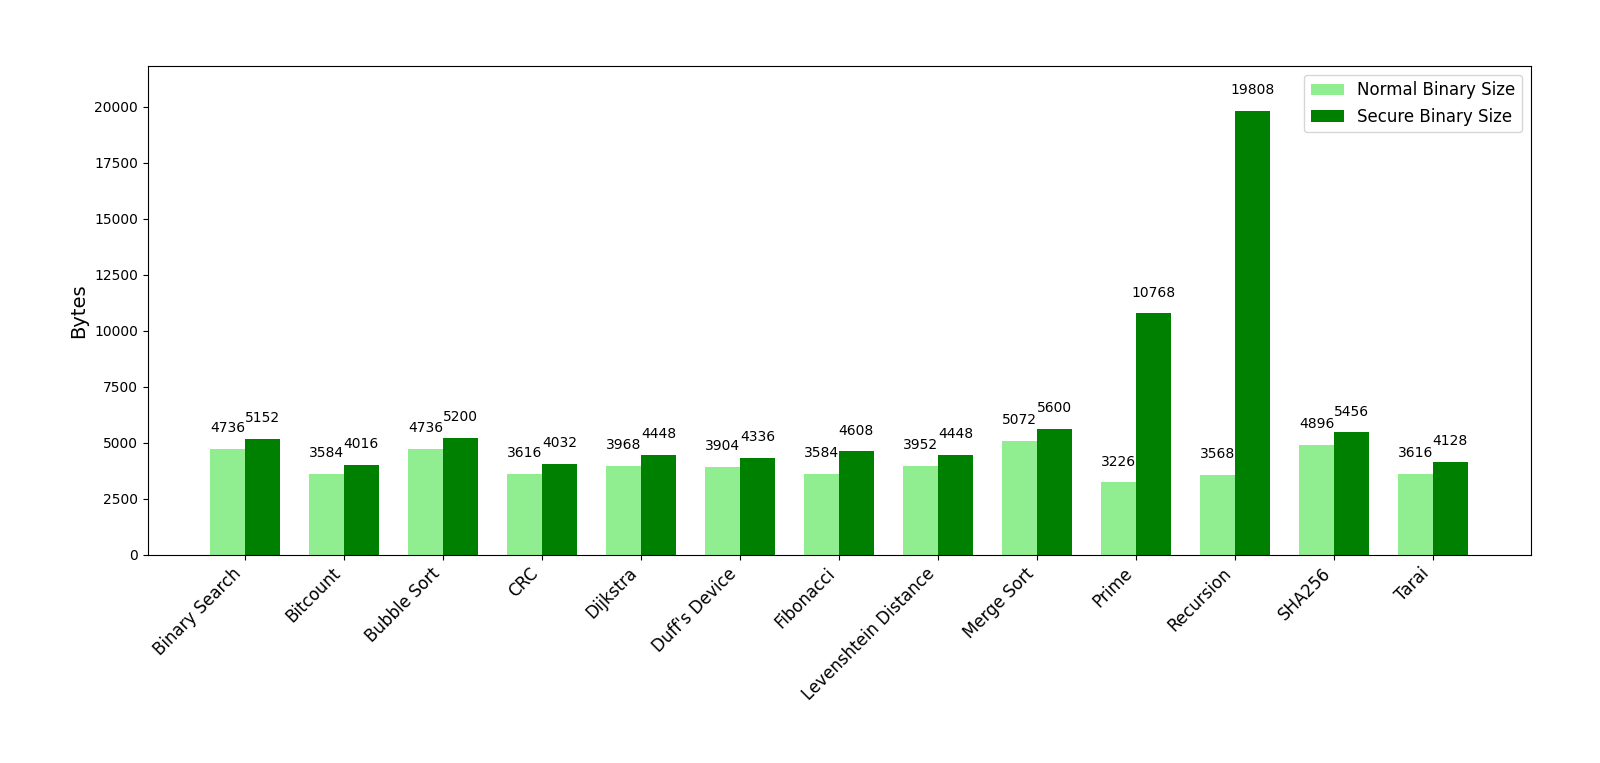
\includegraphics[width=.9\linewidth]{images/bin_sizes.png} } %
  {\scriptsize }
  \caption{Binary sizes}
  \label{fig:binsize}
\end{figure}

\begin{table}
  \centering
  \begin{tabular}{|c|c|c|c|}
    \hline
    \textbf{Algorithm}   & \textbf{Normal bin size (B)} & \textbf{Secure bin size (B)} & \textbf{Memory Overhead} \\
    \hline
    Binary Search        & 4736                         & 5152                         & $8.78\%$                 \\
    \hline
    Bitcount             & 3584                         & 4016                         & $12.05\%$                \\
    \hline
    Bubble Sort          & 4736                         & 5200                         & $9.79\%$                 \\
    \hline
    CRC                  & 3616                         & 4032                         & $11.51\%$                \\
    \hline
    Dijkstra             & 3968                         & 4448                         & $12.09\%$                \\
    \hline
    Duff's Device        & 3904                         & 4336                         & $11.06\%$                \\
    \hline
    Fibonacci            & 3584                         & 4608                         & $28.57\%$                \\
    \hline
    Fibonacci Indirect   & 3600                         & 4064                         & $12.88\%$                \\
    \hline
    Levenshtein Distance & 3952                         & 4448                         & $12.55\%$                \\
    \hline
    Merge Sort           & 5072                         & 5600                         & $10.41\%$                \\
    \hline
    Merge Sort Indirect  & 5088                         & 5600                         & $10.06\%$                \\
    \hline
    Prime                & 3226                         & 10768                        & $233.78\%$               \\
    \hline
    Prime Indirect       & 3712                         & 10768                        & $190.08\%$               \\
    \hline
    Recursion            & 3568                         & 19808                        & $455.15\%$               \\
    \hline
    Recursion Indirect   & 3584                         & 19808                        & $452.68\%$               \\
    \hline
    SHA256               & 4896                         & 5456                         & $11.43\%$                \\
    \hline
    Tarai                & 3616                         & 4128                         & $14.16\%$                \\
    \hline
  \end{tabular}
  \caption{Comparison of binary sizes}
  \label{tab:binsize}
\end{table}

\section{Results and Analysis}
\label{sec:pa_results}

In this section, we will discuss the obtained result and showcase the weak point
of the project. As we have seen in the previous sections the project
performances are not impacting the normal performances of the non-secure binary.
Overall the project suffers an acceptable overhead both in terms of time and space
but has some edge cases where this becomes too big.

In the case of recursive algorithms, we have seen that the time overhead grows
exponentially due to the high number of control transfer functions. Also, the
size of the binary grows as we need a bigger Shadow Stack to store all the
addresses needed to perform the edge controls. However, in the next section, we will
see some optimization techniques that could be applied to the project to reduce the
impact on size and time in these cases.

Moreover, we have seen that if the code is composed of thousands of lines it is
likely that the Control Flow Graph will be very big. This is because if we have many
jump instructions from different sources to different destinations we must store
each pair, thus the space occupied by the CFG grows.

\section{Optimization Techniques}
\label{sec:pa_optimization}

In this section, we will see some optimizations that could be applied to the
project to make it less impactful on the code.

Firstly, in a situation where we need to store a high amount of addresses for a recursive
algorithm, we could modify the Shadow Stack in the following way. If we see that
a function calls itself many times we could store the address one time and,
instead of popping it each time we could just peek at it. In this way, we could
still perform the control but we would need to store the address only once, then
if we need to check a different address we could pop the ``recursive'' address and
then pop the following one to see if it matches the one we are checking. With
such modification, we could effectively reduce the amount of space occupied by the
Shadow Stack without impacting the security features that the project provides.

Lastly, to optimize the Control Flow Graph in peculiar cases (like the aforementioned
firmware one) we could use a Hash Table as already explained in Section
\ref{sec:project_cfg}. As already explained, this solution consumes a lot of
space to prevent collisions but, if the CFG is very big we could at least improve
the time performances.

In conclusion, we have seen that the project offers good performances but it has
some edge cases where it impacts the performances in a severe way. However, it
could be fine-tuned to adapt to such specific situations.
